\documentclass[12pt]{article}
\title{Mapping rainfall anomalies during the 2014-2016 El Ni{\~n}o event}
\author{P. Krishna Krishnamurthy | UCLA ID: 904723392}
\date{}
\usepackage{graphicx}
\usepackage{float}
\usepackage{textcomp}


\begin{document}
\maketitle

\begin{abstract}
There is consensus in the climate science community that El Ni{\~n}o events, periods of anomalously high sea surface temperatures in the Pacific, are associated with disruptions to monsoon patterns which lead to changes in rainfall patterns. The 2014-2016 El Ni{\~n}o episode was an unprecedented event of a scale not seen before, and there is concern that such events may become more frequent under climate change. Understanding rainfall anomalies associated with such large-scale events is the first step towards anticipating potential impacts on vulnerable systems including rain-fed agriculture. Here I utilize remotely-sensed data from the Tropical Rainfall Measurement Mission (TRMM) and the Global Precipitation Measurement Mission (GPM) to illustrate the geographic distributions of rainfall anomalies reported in 2016, at the peak of the recent 2014-2016 Ni{\~n}o event.
\end{abstract}

\section{Introduction}
El Ni{\~n}o events, periods of anomalously high sea surface temperatures in the Pacific, are associated with disruptions to monsoon patterns which lead to changes in rainfall patterns. The 2014-2016 El Ni{\~n}o episode was an unprecedented event of a scale not seen before, and there is concern that such events may become more frequent under climate change \cite{cai2014increasing}. Understanding rainfall anomalies associated with such large-scale events is the first step towards anticipating potential impacts on vulnerable systems including rain-fed agriculture. This information can then be used to understand which societies or systems are particularly vulnerable to strong El Ni{\~n}o episodes, and can be used to prepare risk management strategies \cite{wang2017nino}. 

\section{Materials \& Methods}
\subsection{Data}
The TRMM satellite was launched in November 1997 and terminated operations in April 2015. The satellite provided rainfall information at a high spatial resolution (1 degree  by 1 degree) and very high temporal resolution (every 3 hours) for all coordinates between 60\textdegree N and 60\textdegree S. The GPM was launched in February 2014 building on the successes of TRMM and provides compatibility with TRMM datasets. Data are available for download in 3-hour, 1-day, and 30-day intervals.

Monthly average rainfall rates (measured in terms of mm/hr) were downloaded for the period 1998-2014 from the NASA-TRMM server, and for the period 2015-2016 from the NASA-GPM server. To determine historical rainfall climatology, the average rainfall rate was calculated for the period 1998-2015. A thirty-year dataset is usually considered to be sufficient to establish climatology; unfortunately the historical data are limited so climatology is established using data over a 17-year period. To determine rainfall anomalies in 2016, the difference between the average rainfall values of 2016 and the 17-year historical average was calculated.

However, annual rainfall anomalies only tell part of the story. To better understand the impact of El Ni{\~n}o episodes, it is useful to also consider seasonal rainfall patterns. Seasons were defined as follows: boreal winter (December, January, February), boreal spring (March, April, May), boreal summer (June, July, August), and boreal autumn (September, October, November) following convention in climate science cf. \cite{larkin2005global}. Seasonal anomalies were calculated by first calculating seasonal averages between December 2015 and November 2016, and comparing those to seasonal average rainfall rates between December 1997 and November 2015 (the latter is again considered climatology).      
 
\subsection{Annotated code}
Here I will add all codes used for the project.

Here is some pseudocode for the last code I will need:

\begin{verbatim}
list_of_all_rainfall_values = []
for loop to calculate long-term average:
   using function readPrecip which returns precipitation values
   for file in all_files:
   readPrecip, return precipitation values
   append all precipitation data to list_of_all_values
   return list_of_all_values

add all elements of list and divide by length of list = long_term_mean_precip

using function MapPrecip, map long_term_mean_precip
\end{verbatim}

\section{Results}
Here I will add the final images. Here are some placeholders.

Figure 1 below shows mean rainfall rates for the last quarter of 2015.

\begin{figure}[h]
    \label{fig:meanQ42015}
\centering
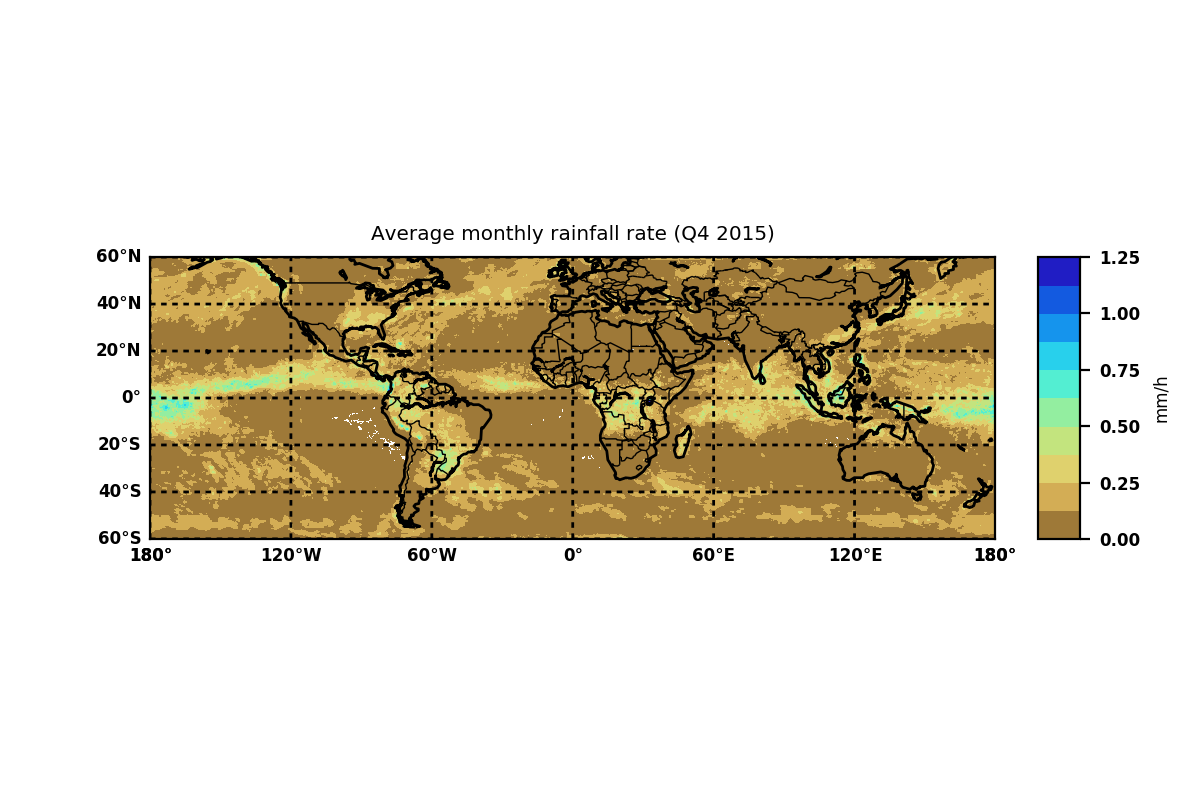
\includegraphics[width=1.25\linewidth]{mean-2015-Q4.png}
\caption{Mean rainfall rates for the last quarter of 2015}
\end{figure}

Figure 2 below shows difference in rainfall between December 2015 and November 2015.

\begin{figure}[H]
    \label{fig:difference}
\begin{center}
   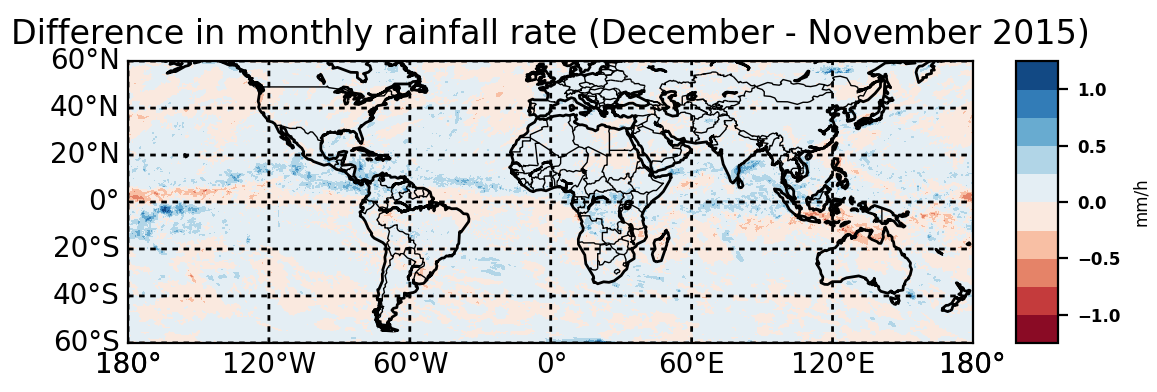
\includegraphics[width=1.25\linewidth]{diff-example.png}
\end{center}
\caption{Difference in rainfall rates between December and November of 2015}
\end{figure}

\bibliography{eeb177.bib}
\bibliographystyle{apalike}

\end{document}
